\documentclass[tikz,border=4pt]{standalone}
\usepackage{ctex}
\usepackage{amsmath}
\usetikzlibrary{arrows.meta}

% p8-04a: 一次函数应用——速度-时间图（v=60, 路程y=60x的图象 + 实际意义）
\begin{document}
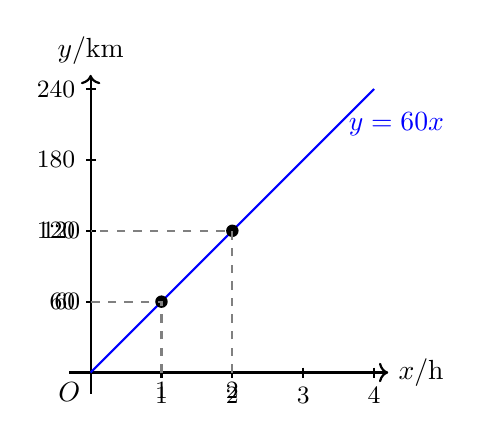
\begin{tikzpicture}[scale=0.9, thick]
  % 坐标轴
  \draw[->] (-0.3,0) -- (4.2,0) node[right] {$x$/h};
  \draw[->] (0,-0.3) -- (0,4.2) node[above] {$y$/km};
  \node[below left] at (0,0) {$O$};

  % 刻度
  \foreach \x in {1,2,3,4} {
    \draw (\x, 2pt) -- (\x, -2pt) node[below] {\small$\x$};
  }
  \foreach \y in {60,120,180,240} {
    \pgfmathsetmacro{\yp}{\y/60}
    \draw (2pt,\yp) -- (-2pt,\yp) node[left] {\small$\y$};
  }

  % 函数 y=60x
  \draw[blue, thick] (0,0) -- (4, 4);
  \node[right, blue] at (3.5, 3.5) {$y=60x$};

  % 具体点
  \fill (1,1) circle (2.5pt);
  \draw[gray, dashed] (1,0) -- (1,1) -- (0,1);
  \node[below] at (1,0) {\small$1$};
  \node[left] at (0,1) {\small$60$};

  \fill (2,2) circle (2.5pt);
  \draw[gray, dashed] (2,0) -- (2,2) -- (0,2);
  \node[below] at (2,0) {\small$2$};
  \node[left] at (0,2) {\small$120$};
\end{tikzpicture}
\end{document}
